\documentclass[11pt,a4paper]{article}
\usepackage[a4paper,margin=28mm]{geometry}
\usepackage[T1]{fontenc}
\usepackage[utf8]{inputenc}
\usepackage{lmodern}
\usepackage{amsmath,amssymb,amsthm}
\usepackage{graphicx,booktabs,xcolor,hyperref}
\usepackage[backend=biber,style=numeric,sorting=none]{biblatex}
\addbibresource{references.bib}
\DeclareFieldFormat{doi}{\url{https://doi.org/#1}}
\hypersetup{colorlinks=true,linkcolor=black,citecolor=black,urlcolor=black,pdfborder={0 0 0},hypertexnames=false}
\providecommand{\Description}[1]{}
\usepackage{amsmath,amssymb,amsthm,mathtools,tabularx,array,needspace,booktabs}
\usepackage{enumitem,listings,xurl,graphicx,microtype,float}
\usepackage{tikz}
\usetikzlibrary{arrows.meta,positioning,calc,intersections}
\usepackage[nameinlink,noabbrev]{cleveref}
\newtheorem{theorem}{Theorem}[section]
\newtheorem{lemma}[theorem]{Lemma}
\crefname{lemma}{Lemma}{Lemmas}
\newtheorem{proposition}[theorem]{Proposition}
\newtheorem{corollary}[theorem]{Corollary}
\theoremstyle{definition}
\newtheorem{definition}[theorem]{Definition}
\newtheorem{remark}[theorem]{Remark}
\newcommand{\R}{\mathbb R}
\newcommand{\I}{\{0,1,\ldots,10\}}
\newcommand{\orient}{\operatorname{orient}}
\newcommand{\CCW}{\operatorname{StrictCCW}_{11}}
\newcommand{\CertCheck}{\operatorname{Check}}
\newcommand{\Cand}{\operatorname{Cand}}
\newcommand{\code}[1]{\texttt{#1}}
\lstset{basicstyle=\footnotesize\ttfamily,columns=fullflexible,keepspaces=true,
 breaklines=true,frame=single,framerule=.25pt,rulecolor=\color{black!20},
 backgroundcolor=\color{black!2},aboveskip=7pt,belowskip=7pt}
\setlength{\emergencystretch}{1em}
\raggedbottom
\hypersetup{pdftitle={An End-to-End Lean Verification of the Eleven-Vertex Case of Erdos Problem 97},pdfauthor={Dang Khoa Nguyen}}
\title{An End-to-End Lean Verification of the Eleven-Vertex Case of Erd\H{o}s Problem 97}
\author{Dang Khoa Nguyen\\[2pt]
\small Vietnam--Japan Institute of Technology\\
\small Ho Chi Minh City University of Technology (HUTECH)\\
\small Ho Chi Minh City, Vietnam\\[3pt]
\small ORCID: \href{https://orcid.org/0009-0005-3242-0098}{0009-0005-3242-0098}\\[2pt]
\small Corresponding author: \href{mailto:shirakawa.ryouya.work@gmail.com}{\nolinkurl{shirakawa.ryouya.work@gmail.com}}}
\date{}
\begin{document}
\maketitle
\begin{abstract}
We establish the eleven-vertex case of the four-equidistant-neighbours question associated with Erd\H{o}s Problem 97. For any eleven planar points in strictly convex counterclockwise order, some vertex has at most three other vertices at every fixed distance from it; the distance may vary with the vertex. A hypothetical counterexample selects four equidistant witnesses at each centre. Proved geometric restrictions, strict quadrilateral inequalities, and a verified tree checker exclude every such selection. The Lean 4.36.0-rc1 development closes the geometric reduction, two finite-table certifications, 210 root cases, and the final theorem without a certificate-acceptance hypothesis. The final axiom audit reports only \code{propext}, \code{Classical.choice}, and \code{Quot.sound}. A staged clean replay compiled all 680 project modules from pinned sources without importing the earlier release's project objects. The original certificate forest has 5,246,380 nodes. The contribution is a closed formal verification for exactly eleven vertices, rather than a new general-purpose search algorithm or a resolution of the unrestricted question, for which large-cardinality counterexamples have been announced.
\end{abstract}
\noindent\textbf{Keywords:} convex polygons; equidistant vertices; Erd\H{o}s Problem 97; Lean; formal verification; proof certificates
\section{Introduction and relation to earlier work}\label{sec:intro}
For a finite set $V\subset\R^2$, a vertex $p\in V$ is \emph{four-rich} if some circle of positive radius centred at $p$ contains at least four other points of $V$. Erd\H{o}s Problem 97 asks whether every convex polygon has a vertex that is not four-rich. The radius may vary with the centre. A counterexample requires every vertex to have four equidistant neighbours, but does not require one common radius for the entire polygon.

The question originates in the distance problems of Erd\H{o}s~\cite{Erdos1946,Erdos1987}. His earlier three-neighbour conjecture was refuted by Danzer's nine-vertex construction, described in \cite{Erdos1987}. Fishburn and Reeds~\cite{FishburnReeds1992} obtained a twenty-vertex example with a common unit radius. Neither example supplies four neighbours. Bounds on the number of distinct distances from a vertex~\cite{Dumitrescu2006,Nivasch2013} address a related statistic; a lower bound on the number of distinct radii does not by itself bound every radius multiplicity by three.

Recent computational work provides especially relevant comparisons. The public ten-vertex repository\footnote{\raggedright \url{https://github.com/veljjanoski/erdos97}; repository commit 1aed58e2da4cfcd54cf37c367293a9eb3be9042b.} reports exclusion of strictly convex counterexamples with at most ten vertices, using incidence enumeration and exact polynomial calculations. Its ten-vertex result uses Gr\"obner-basis computations and its stated scope leaves eleven vertices unresolved. A separate research ledger\footnote{\raggedright \url{https://github.com/davidiach/erdos97}; source version d269911b92e465f1062e72160d6ade0563c4a4fb.} records local small-case results and restricted-family investigations. These are cited as author-reported computational results; we have not independently replayed their complete calculations. The numerical experiments described in Problem 6.53 of Georgiev et al.\footnote{\raggedright Preprint: \url{https://arxiv.org/abs/2511.02864v3}.} also considered the four-neighbour question without producing a counterexample.

Kruer, Kohlmeyer, and Price\footnote{\raggedright Public manuscript and source: \url{https://github.com/lkruer/erdos-96-97-proof/blob/0e98f5f9bdaf36007e3eb405cbefe2eda778a9b2/96-97.tex}.} have made public a manuscript claiming strictly convex configurations of all sufficiently large cardinalities with at least four \emph{unit-distance} neighbours at each vertex, together with a Lean formalization. This provides a claimed negative answer to the unrestricted question. We report the stated scope of that public work without asserting that we have independently replayed its proof. A positive assertion at the specific size eleven is entirely compatible with sufficiently large counterexamples.

\paragraph{Contribution and novelty boundary.}
The result here is a size-specific, fully closed Lean theorem at $n=11$. In relation to the reported exclusions through ten vertices (see \Cref{sec:intro}), it addresses the next finite case without relying on those external computations. Its additional formal-methods contribution is an end-to-end dependency chain: Euclidean witness selection, sound geometric pruning, certified finite tables, exhaustive tree coverage and a theorem with no residual table-acceptance premise. The finite certificate producer is untrusted; the checker and its soundness bridge are part of the verified development. The original forest's size also makes the compilation and proof-carrying packaging techniques relevant to reproducibility. We do not claim invention of certificate checking, double counting, proof by exhaustive search, or opaque declarations. We use Lean~\cite{Lean2021} and mathlib~\cite{Mathlib2020}; the standard finite-set conjecture interface is a separate formulation\footnote{\raggedright \url{https://github.com/google-deepmind/formal-conjectures/blob/7db2ea3b91bfbd0ab620215163e6c488bbb916d5/FormalConjectures/ErdosProblems/97.lean}}.


\subsection{Why this is a formal reasoning case study}
The obstacle to a proof at eleven vertices is not the number of
choices alone. An arbitrary finite search could report that no
assignment survives, yet fail to establish a geometric theorem:
a row enumeration might omit a witness set; a pruning predicate
might reject a realizable pair; a certificate might omit a branch;
or an imported acceptance condition could remain in the final
statement. These are distinct proof obligations. The development
addresses them by proving the connection between Euclidean
geometry and decoded rows, checking each exclusion reason,
showing that realized rows survive filtering, checking every child
of a branching node, and applying the resulting exhaustive root
certificates to the closed theorem. The claims concern this
particular development, not a general completeness theorem for
certificate-producing searches.

\paragraph{What can be reused and what cannot.}
The proof separates an untrusted heuristic producer from a
trusted, independently specified Boolean checker with a proved
soundness theorem. Equality-walk receipts are small local
explanations for strict-metric contradictions. The source also
illustrates how proof-carrying opaque values can keep unusually
large certificate expressions from being unfolded throughout an
assembly proof. We present these as engineering lessons and
inspectable design choices rather than as a newly invented
inference system. Neither the finite search nor the closed
$n=11$ theorem yields an induction argument for arbitrary $n$.

\section{The theorem and its formal scope}\label{sec:statement}
Write $P_i=(x_i,y_i)$ and put
\[
 \begin{gathered}\orient(a,b,c)=\det(b-a,c-a),\\ D_{ij}=(x_i-x_j)^2+(y_i-y_j)^2.\end{gathered}
\]
The formal hypothesis on $P:\I\to\R^2$ is
\begin{equation}\label{eq:ccw}
 \begin{gathered}\CCW(P)\quad\Longleftrightarrow\\ \orient(P_i,P_j,P_k)>0\quad(0\le i<j<k\le10).\end{gathered}
\end{equation}
It refers to all increasing triples, not merely consecutive triples. For vertices of a strictly convex polygon in counterclockwise order, \eqref{eq:ccw} holds. Conversely, the cyclically ordered list satisfying \eqref{eq:ccw} is in strictly convex position: every directed successive edge has all other points strictly to its left. This includes the last edge by cyclic invariance of orientation. In particular the points are distinct and no three are collinear.

\begin{theorem}[Eleven-vertex case]\label{thm:main}
Let $P_0,\ldots,P_{10}\in\R^2$ satisfy \eqref{eq:ccw}. Then
\begin{equation}\label{eq:main}
 \begin{gathered}\exists c\in\I\;\forall r>0,\qquad\\
 \bigl|\{j\in\I\setminus\{c\}:\|P_j-P_c\|=r\}\bigr|\le3.\end{gathered}
\end{equation}
\end{theorem}
The kernel-checked declaration is \path{T34Closed.erdos97_n11_strict_ccw}. Its literal conclusion is the equivalent finite-witness statement
\begin{equation}\label{eq:formal}
 \begin{gathered}\exists c\in\I\;\forall W\subseteq\I\setminus\{c\},\quad |W|=4\\
 \Longrightarrow\quad \neg\bigl(\forall u,v\in W,\ D_{cu}=D_{cv}\bigr).\end{gathered}
\end{equation}
If \eqref{eq:main} fails at this $c$, choose four points on the offending circle to contradict \eqref{eq:formal}. Conversely four witnesses in \eqref{eq:formal} would have a positive common distance, since the points are distinct. This proves the mathematical equivalence of the two forms. The release does not add a separate Lean wrapper in the \code{ConvexIndep} interface mentioned in \Cref{sec:intro}; its checked contract is explicitly \eqref{eq:ccw} and \eqref{eq:formal}.

The theorem imposes no rationality, regularity, cyclicity, or symmetry assumption. Coordinates range over all real numbers. It does not claim the result for every cardinality, for redundant collinear boundary points, or for arbitrary non-convex sets. Nor does it by itself prove all smaller cardinalities: deleting a vertex can destroy a four-witness set at another centre.

\section{From geometry to finite witness assignments}\label{sec:geometry}
\subsection{Rows and their geometric meaning}
Suppose every vertex is four-rich. For each centre $c$, select a set $S_c\subset\I\setminus\{c\}$ of cardinality four with
\begin{equation}\label{eq:row}
 D_{cu}=D_{cv}\quad(u,v\in S_c).
\end{equation}
There are $\binom{10}{4}=210$ possible sets at each centre. Enumerating them lexicographically gives row identifier $210c+k$, $0\le k<210$, hence 2,310 rows. The enumeration-to-geometry bridge is itself proved: any four-rich configuration produces a complete assignment of one valid row per centre. The proof does not require a numerical search over coordinates.

There are $\binom{11}{2}=55$ unordered edges. Give edge $\{i,j\}$ the nonnegative length $\ell_{ij}=\sqrt{D_{ij}}$. A selected row makes its four spoke lengths equal. This passage applies the same square-root function to equal squared distances. The linear inequalities below concern $\ell_{ij}$, not $D_{ij}$.


\begin{figure}[tbp]
\centering
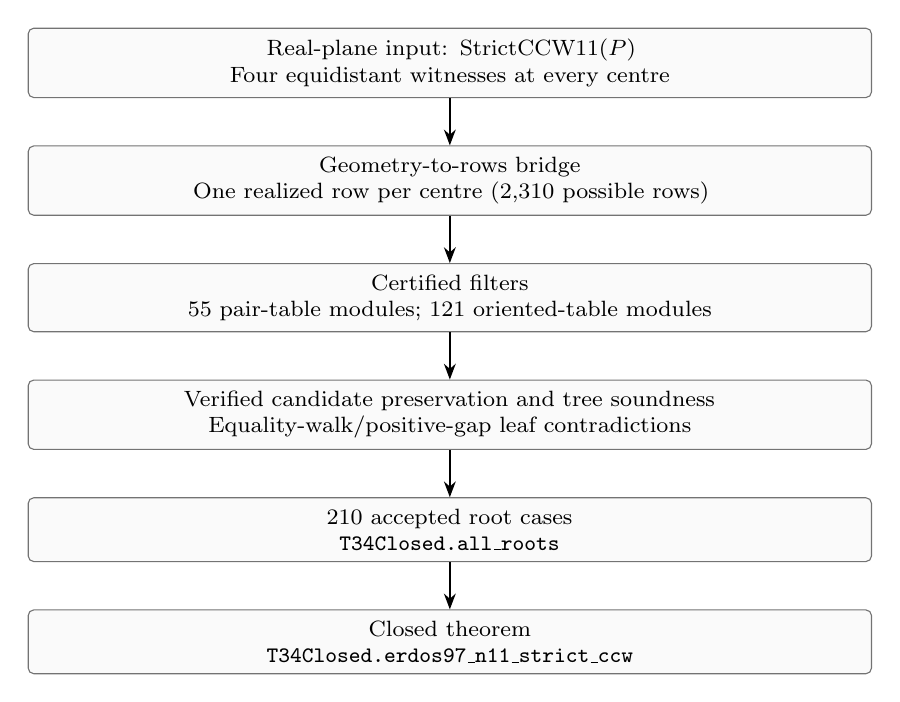
\begin{tikzpicture}[>=Stealth,node distance=6mm,
  every node/.style={font=\footnotesize,align=center},
  unit/.style={draw=black!55,rounded corners=2pt,text width=.86\linewidth,
    minimum height=8mm,inner sep=4pt,fill=black!2}]
\node[unit] (a) {Real-plane input: $\mathrm{StrictCCW11}(P)$\\Four equidistant witnesses at every centre};
\node[unit,below=of a] (b) {Geometry-to-rows bridge\\One realized row per centre (2,310 possible rows)};
\node[unit,below=of b] (c) {Certified filters\\55 pair-table modules; 121 oriented-table modules};
\node[unit,below=of c] (d) {Verified candidate preservation and tree soundness\\Equality-walk/positive-gap leaf contradictions};
\node[unit,below=of d] (e) {210 accepted root cases\\\texttt{T34Closed.all\_roots}};
\node[unit,below=of e] (f) {Closed theorem\\\texttt{T34Closed.erdos97\_n11\_strict\_ccw}};
\foreach \x/\y in {a/b,b/c,c/d,d/e,e/f}{\draw[->,line width=.6pt] (\x.south)--(\y.north);}
\end{tikzpicture}
\caption{Proof architecture of the frozen development. Every arrow denotes
an implication implemented in the Lean dependency chain; the
external C++/Python certificate producer is not a logical premise.}
\label{fig:architecture}
\end{figure}

\subsection{Two-centre and three-centre restrictions}
\begin{lemma}[Shared witnesses]\label{lem:shared}
For two distinct centres $a,b$, their selected sets have at most two common witnesses. If $u,v$ are distinct common witnesses, the chord $P_uP_v$ crosses the chord $P_aP_b$ in their relative interiors.
\end{lemma}
\begin{proof}
The witnesses lie at intersections of two circles with distinct centres, which have at most two intersection points. When there are two, they are reflections of each other across the line through the centres and lie strictly on opposite sides of that line. For vertices of a strictly convex polygon this gives alternation of $u,v$ across the two arcs separated by $a,b$, equivalently chord crossing. The coordinate implementation derives the conclusion from perpendicular-bisector identities and orientation signs.
\end{proof}
\begin{lemma}[Pair capacity]\label{lem:paircapacity}
A fixed pair of distinct witnesses $u,v$ belongs to selected sets at at most two distinct centres.
\end{lemma}
\begin{proof}
Every such centre lies on the perpendicular bisector of $P_uP_v$. Three distinct centres would be collinear, contradicting \eqref{eq:ccw}.
\end{proof}
If $d(v)=|\{c:v\in S_c\}|$, count pairs $(c,u)$ with $v,u\in S_c$ and $u\ne v$. Each selected set containing $v$ contributes three pairs; each other label $u$ contributes at most two. Therefore
\begin{equation}\label{eq:incoming}
 3d(v)\le2(11-1)=20,\qquad d(v)\le6.
\end{equation}
The implemented three-row pruning test verifies an actual pair-capacity violation; it does not trust an unverified integer counter.

\subsection{A five-point obstruction}\label{sec:fivepoint}
The pair table also uses the following obstruction and its reflected version. We include the proof to expose this filter's algebraic content.
\begin{lemma}[Five-point obstruction]\label{lem:five}
Let $P,A,B,C,Q$ occur in this cyclic order in strictly convex position. It is impossible to have
\begin{equation}\label{eq:five}
 |BP|=|BA|,\qquad |CQ|=|CA|,\qquad |CA|\le |CB|.
\end{equation}
\end{lemma}
\begin{proof}
Apply an orientation-preserving similarity taking $A$ to $(0,0)$ and $B$ to $(1,0)$. Write $P=(x,y)$, $C=(t,h)$, $Q=(u,v)$. The cyclic orientation conditions imply
\begin{gather*}
 y,h,v>0,\quad uy-vx>0,\quad tv-hu>0,\\
 z:=h(1-u)-(1-t)v>0.
\end{gather*}
The distance conditions give
\[
 \begin{gathered}2x-x^2-y^2=0,\quad 1-2t\ge0,\\
 E:=u^2+v^2-2tu-2hv=0.\end{gathered}
\]
The first identity and $y>0$ imply $x>0$; then $uy-vx>0$ implies $u>0$, and $tv-hu>0$ implies $t>0$. The identity
\[
 2h-v=2z+2hu+(1-2t)v
\]
gives $2h-v>0$. Finally direct expansion yields
\begin{equation}\label{eq:fiveidentity}
 hE+u(tv-hu)+(ut+hv)(2h-v)=0.
\end{equation}
The first term is zero and the other two are strictly positive. The formal proof uses a polynomial rotation-and-scaling map with $B=(d,0)$, $d>0$, to avoid normalization by a square root; \eqref{eq:fiveidentity} is unchanged.
\end{proof}
For example a row at $B$ containing $P,A$, together with a row at $C$ containing $Q,A,B$, forces \eqref{eq:five}. Reversing cyclic order and reflecting gives the companion forbidden pattern: a row at $A$ contains $P,B,C$, and a row at $B$ contains $Q,C$. All cyclic placements are transported from the proved geometric statements to the actual decoded masks.

\subsection{Strict quadrilateral gaps}
\begin{lemma}[Crossing-diagonal inequalities]\label{lem:quad}
If $i<j<k<l$, then
\begin{align}
 g^{(0)}_{ijkl}&:=\ell_{ik}+\ell_{jl}-\ell_{ij}-\ell_{kl}>0,\label{eq:quad0}\\
 g^{(1)}_{ijkl}&:=\ell_{ik}+\ell_{jl}-\ell_{il}-\ell_{jk}>0.\label{eq:quad1}
\end{align}
\end{lemma}
\begin{proof}
The diagonals meet at an interior point $X$. Strict triangle inequalities give $|P_iP_j|<|P_iX|+|XP_j|$ and $|P_kP_l|<|P_kX|+|XP_l|$. Adding and using additivity along diagonals proves \eqref{eq:quad0}; the other sides prove \eqref{eq:quad1}. The formal development proves that both intersection parameters lie in $(0,1)$ from orientation signs before applying the metric argument. These are strict Euclidean forms of the Kalmanson inequalities~\cite{Kalmanson1975}.
\end{proof}
\begin{figure}[tb]
\centering
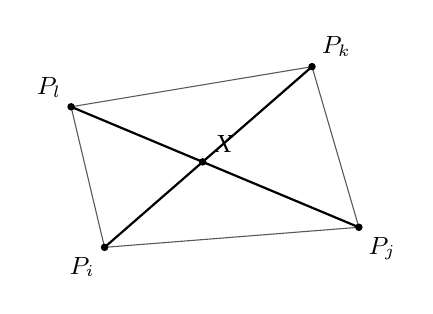
\begin{tikzpicture}[scale=.85,every node/.style={font=\small}]
\coordinate (A) at (0,0);\coordinate (B) at (3.8,.3);
\coordinate (C) at (3.1,2.7);\coordinate (D) at (-.5,2.1);
\draw[black!65] (A)--(B)--(C)--(D)--cycle;
\draw[black,thick,name path=AC] (A)--(C);
\draw[black,thick,name path=BD] (B)--(D);
\path[name intersections={of=AC and BD,by=X}];
\fill (X) circle(1.6pt);\node[above right] at (X){$X$};
\foreach \p/\lab/\pos in {A/i/below left,B/j/below right,C/k/above right,D/l/above left}
{\fill (\p) circle(1.6pt);\node[\pos] at (\p){$P_{\lab}$};}

\end{tikzpicture}
\caption{The strict geometric inequality used by a flow certificate. Squared distances encode row equalities; gaps use ordinary lengths.}\label{fig:quad}

\end{figure}
There are $2\binom{11}{4}=660$ gaps. A finite shape check proves that every table entry has the stated form; it is then connected to Lemma~\ref{lem:quad}.

\section{Certificates and a verified rejection procedure}\label{sec:checker}
\subsection{Certified tables and candidate lists}
A \emph{prefix} $p$ is a list of selected row identifiers. The two-centre compatibility table has $55\cdot210^2=2,425,500$ slots. A forbidden slot supplies a nonzero reason code validated against Lemmas~\ref{lem:shared} and~\ref{lem:five}. A zero code is not accepted as evidence of rejection. The table is certified in 55 centre-pair modules. An oriented representation stores a 210-bit mask for a fixed row and target centre; its 121 ordered centre-pair blocks are separately certified against the first table.

For target centre $c$, intersect the masks for all rows in $p$. Filter the remaining row identifiers using checked hints for Lemma~\ref{lem:paircapacity}. Denote the resulting list by $\Cand(p,c)$. The crucial preservation property is
\begin{equation}\label{eq:survival}
\begin{gathered}
 \text{$P$ realizes a complete assignment $a$}\\
 \text{and realizes $p$}\\
 \Longrightarrow\quad a(c)\in\Cand(p,c)\qquad(c\in\I).
\end{gathered}
\end{equation}
It holds for any supplied hint provider because each used rejection is checked. An incomplete hint can slow the search but cannot discard a genuine assignment. The two table certifications are explicit hypotheses of intermediate soundness theorems and are discharged in the final theorem.

\subsection{Equality walks and positive-gap contradictions}
Each row makes four edge lengths equal. An \emph{equality walk} from edge $e$ to edge $f$ consists of steps $(r,e')$ using a row $r$ in the prefix, with both the current edge and next edge $e'$ among its spokes. Transitivity gives $\ell_e=\ell_f$.

A flow certificate lists a nonempty family of gaps $g_q$ with positive integer weights $w_q$. Expand
\begin{equation}\label{eq:flow}
 G=\sum_q w_qg_q
\end{equation}
as a multiset of positive edge occurrences minus a multiset of negative edge occurrences. The certificate gives one equality walk from each positive occurrence to a negative occurrence. The checker verifies the walks and that their endpoint multiset is exactly the entire negative multiset. Hence $G=0$. But Lemma~\ref{lem:quad} and the positive weights give $G>0$.

Weights are checked as positive natural numbers, bounded by $10^6$ in the implementation. Gap indices are range-checked. This uses exact integer arithmetic and equality of finite lists, without a numerical tolerance or trust in the producer's optimization routine.

\paragraph{A small extracted example.}
One leaf of root 0, at token offset 28, uses rows
\[
 \begin{gathered}(0;1,2,3,4),\quad (9;1,5,7,8),\\
 (10;0,4,5,6).\end{gathered}
\]
The two gaps
\begin{align*}
 g_{609}&=\ell_{4,9}+\ell_{5,10}-\ell_{4,10}-\ell_{5,9},\\
 g_{38}&=\ell_{0,4}+\ell_{1,9}-\ell_{0,1}-\ell_{4,9}
\end{align*}
are positive. Their sum is zero because the rows imply, respectively,
$\ell_{0,4}=\ell_{0,1}$, $\ell_{1,9}=\ell_{5,9}$, and
$\ell_{5,10}=\ell_{4,10}$. This is an ordinary short proof of this leaf;
it does not replace coverage of the remaining cases.


\paragraph{Why this example is a proof, not a numerical test.}
Using only cancellation and the row equalities above, the two
strictly positive gaps satisfy
\[
\begin{aligned}
 g_{609}+g_{38}
  ={}&(\ell_{5,10}-\ell_{4,10})
  +(\ell_{1,9}-\ell_{5,9})\\
   &+(\ell_{0,4}-\ell_{0,1})=0.
\end{aligned}
\]
The contradiction is $0=g_{609}+g_{38}>0$. In a full certificate,
this cancellation is not taken on faith: every asserted equality
between edge lengths is supplied as a walk whose individual
steps are checked against the currently selected rows. The checker
also matches the complete multiset of negative edge occurrences;
showing only a subset of cancellations would not justify acceptance.
The displayed example demonstrates one particular leaf, not a
shortcut for enumerating or accepting the entire forest.

\subsection{Tree nodes and coverage}
The certificate datatype has three constructors:
\begin{enumerate}[label=(\roman*)]
\item \emph{flow}: an equality-walk contradiction;
\item \emph{empty}: a centre whose recomputed candidate list is empty;
\item \emph{branch}: a centre and one child for each row in its candidate list.
\end{enumerate}
At a branch, the child-label list must be literally equal to $\Cand(p,c)$, and every child is checked on its extended prefix. Stored masks must equal recomputed intersections. A fuel parameter bounds recursion; zero fuel rejects. These conditions prevent omission of an alternative.

\begin{proposition}[Tree soundness]\label{prop:sound}
Assume the two table certifications. If $\CertCheck(f,p,C)=\mathrm{true}$, no complete geometric witness assignment under \eqref{eq:ccw} realizes $p$.
\end{proposition}
\begin{proof}
Induct on $f$. At zero fuel the check is false. A flow node gives \eqref{eq:flow}. At an empty node, \eqref{eq:survival} supplies a member of the empty list. At a branch it places the assignment's row among the explicitly listed children. Extend the realized prefix and apply the induction hypothesis.
\end{proof}
The producer can choose branch centres and search order heuristically. Soundness needs neither optimal choices nor trust in a search status message. The naive $210^{11}$ assignments are covered through certified pruning and case splitting, not by interpreting a numerical failure to find coordinates as proof.


\subsection{What each Boolean acceptance test must establish}
\Cref{prop:sound} is only useful if the checker has no accepting
shortcut for which the inductive argument is invalid. The
following obligations identify the trust boundary in concrete
terms.\begin{enumerate}[label=(\alph*),leftmargin=*]
\item \emph{Row coverage}: the geometric witnesses of a purported
counterexample map to enumerated row identifiers.
\item \emph{Pair and triple pruning}: any forbidden-code or hint
rejection has a geometric justification; mere nonzero bits or an
external producer verdict are insufficient.
\item \emph{Candidate preservation}: the selected row of a realized
assignment remains in the recomputed candidate list.
\item \emph{Flow leaves}: positive integer weights and every
edge-equivalence step are checked; exact multisets of endpoints
force cancellation of positive gaps.
\item \emph{Empty and branch nodes}: an empty candidate list is
recomputed; a branch's children have exactly the recomputed
candidate labels, rather than a convenient subset.
\item \emph{Termination}: fuel exhaustion rejects rather than
accepts a certificate. The root certificates are accepted with
stated fuel and frozen inputs.
\end{enumerate}
These are the checks represented in the source by the declarations
listed in \Cref{tab:formal-map}. The proof does not require that a
certificate producer is correct or that its search is complete on
arbitrary inputs; only accepted, exhaustively branched certificates
suffice for this instance.

\section{Closing the Lean proof}\label{sec:lean}
Fix centre 0. Its 210 possible rows give every root case, without a symmetry assumption or quotient. The release supplies
\begin{equation}\label{eq:roots}
 \begin{gathered}\forall k<210\;\exists C_k,\qquad\\
 \CertCheck(12,[k],C_k)=\mathrm{true}.\end{gathered}
\end{equation}
\begin{proof}[Proof of Theorem~\ref{thm:main}]
If the conclusion failed, finite witness selection would give a complete assignment. Its row at centre 0 is some $k<210$, so it realizes $[k]$. The certified tables, \eqref{eq:roots}, and Proposition~\ref{prop:sound} contradict this assignment. Negating the counterexample property yields \eqref{eq:formal}, hence \eqref{eq:main}.
\end{proof}
The final term applies the proved assembly theorem to actual certifications:
\begin{lstlisting}
T34EndToEnd.no_counterexample_of_roots
  T32CompleteTable.certified
  T33CompleteTable.certified
  T34Closed.all_roots
\end{lstlisting}
Thus \code{hcheck}, \code{Certified}, and \code{RootsVerified} are not remaining assumptions of the public theorem. This is the sense in which verification is end-to-end.

\subsection{Large certificates and opaque packages}
Most roots were checked directly in the V34 pipeline. Roots 26 and 27 were split into 75 and 90 leaf modules, respectively, then assembled into public declarations with the same namespaces as the other cases. For root 27 a proof-carrying opaque package stores a certificate and its acceptance proof:
\begin{lstlisting}
opaque packed :
  {C : Certificate // checkTree fuel hints prefix C = true} :=
  Subtype.mk leaf leaf_ok
\end{lstlisting}
The parent uses \code{packed.val} and \code{packed.property}. Opacity controls definitional expansion of certificate data; the body and acceptance theorem remain type-checked. It adds no axiom of certificate acceptance. The root-27 representation differs from the old transparent constructor expression, so it has a separate source/object manifest; old frozen manifests are preserved.

In the original V38 distributed run, root-27 assembly took 63.10 seconds after its 90 leaves were checked. The public root-26 wrapper took 2.57 seconds and final closed-theorem compilation 49.70 seconds. These are recorded module durations, not full search or verification times. An earlier root-27 assembly was cancelled before completion; its cause is not established, and it is not a controlled performance comparison.

\subsection{Verification boundary}
The axiom audit reports exactly \code{propext}, \code{Classical.choice}, and \code{Quot.sound} for the closed theorem and assembly declarations. It reports no \code{sorryAx}, custom geometric axiom, or native-evaluation axiom. Finite checks use kernel reduction; \code{native\_decide} is not used to discharge the result. The C++ producer, Python controllers, scheduler, and checksums organize evidence; the mathematical conclusion comes from the checked definitions and proof terms. CRC and SHA256 establish artifact integrity, not logical soundness by themselves.

The plane, orientation, squared-distance and selected-row definitions were inspected against \cref{sec:statement}. We report ordinary Lean source compilation with axiom and dependency audits; no independent external-kernel or comparator replay is claimed. These distinctions follow the verification levels in the Lean reference\footnote{\raggedright \url{https://lean-lang.org/doc/reference/latest/ValidatingProofs/}.}.


\subsection{The trusted base and limits of the evidence}
The kernel-checked claim is the literal Lean declaration, not an
informal assertion that all convexity conventions are interchangeable.
The equivalence between the \code{StrictCCW11} hypothesis and the
stated geometry is explained mathematically in
\Cref{sec:statement}; no direct \code{ConvexIndep} wrapper is part
of the frozen release. A report of successful compilation and an
axiom list is distinct from a second party running an independent
kernel or checking the proof manually. The source and artifact
checks reported below establish traceability and reproducibility,
not independence of verification. Theoretical soundness comes
from the Lean proofs of the geometric bridges, certified tables,
checker invariants and final assembly under the pinned environment.

\section{Artifact and descriptive measurements}\label{sec:measurements}
The environment is Lean 4.36.0-rc1, compiler commit
\nolinkurl{c9afcddf514a6772bd4d649f7cfc04eff0b9f15e}, with mathlib revision
\nolinkurl{625d8914199bc567cca9b91f90e8e5afafa5ae51}.
The original distributed verification used at most sixteen Lean workers, each requesting four CPUs and 4,096 MiB memory; the platform could allocate additional memory. Requested resources are not measurements of actual utilization. We do not infer a total CPU-hour or dollar cost from those requests.

\begin{table}[htbp]
\centering\caption{Audited release and original producer forest. Forest counts describe frozen tokens, not the graph of compiled proof objects.}\label{tab:counts}
\begin{tabular}{lr}\toprule
Quantity & Count\\\midrule
Accepted root cases & 210 / 210\\
Unordered compatibility-table modules & 55 / 55\\
Oriented-table modules & 121 / 121\\
Verified source/object module pairs & 680\\
Original forest nodes & 5,246,380\\
Flow leaves & 3,906,221\\
Empty-candidate leaves & 328,193\\
Branch nodes & 1,011,966\\
Maximum depth below root prefix & 7\\
Original token bytes & 377,654,934\\\bottomrule
\end{tabular}
\end{table}
A read-only replay parsed all 210 token files, checked their SHA256 hashes, node totals and subtree end offsets, and collected \cref{tab:counts}. It is descriptive and does not repeat the kernel proofs. Of the flow leaves, 3,899,879 use at most two listed quadrilateral terms (99.84\%), and 3,638,533 use at most four distinct rows in their equality walks (93.15\%). The latter counts used rows, not all prefix rows. These percentages do not measure the proportion of verification time that can be removed.

\begin{samepage}
The original V38 evidence archive is
\begin{center}\small\path{Erdos97_Lean_EndToEnd_n11_StrictCCW11_V38_20261025.zip},\end{center}
of size 7,737,985,716 bytes and SHA256
\begin{quote}\small\nolinkurl{2c7219ac121a05750ea87a86bb8b5fc813b2565f6f1706f914f3e107c764c621}.\end{quote}
\end{samepage}
It contains primary, parallel, and final-closure components, mappings, kernel logs, frozen inputs and complete file inventories. The collection audit verified all listed member hashes and CRCs. Accompanying source-only material omits compiled project objects, retaining sources, tokens, pinned dependencies, build order and scripts. The original archive remains unchanged; the completed clean replay below supplies separate evidence for rebuilding those sources.

\subsection{Completed clean source replay}\label{sec:clean-replay}
The replay chain \code{clean41-20261025} started with no project objects from the original V38 release. It completed all 680 modules, including the 210 canonical roots and the closed final theorem, on 2 November 2026 (UTC+7). Sources, certificate tokens, the Lean compiler and all nine dependency revisions were pinned. A dependency object was reused only after being built and source/object-verified in this same clean chain. This was a staged rebuild with audited continuations, not a single uninterrupted invocation and not a replay by an independent researcher or a different kernel.

Each accepted module has a successful compilation receipt, its frozen source hash, the resulting object's hash, and the source/object hashes of its full transitive dependency closure. Interrupted reductions, uncompleted attempts and memory snapshots are not counted as successful modules. The last compilation imported 679 such verified objects and built \path{EndToEnd_Closed_V38.lean}; its 18.50-second duration is not the duration of the full rebuild.

\begin{table}[htbp]
\centering\caption{Selected measurements from successful modules in the clean replay. Elapsed times are per module; RSS is the peak sampled resident memory of its Lean process.}\label{tab:clean-replay}
\begin{tabular}{lr}\toprule
Quantity & Measurement\\\midrule
Completed source/object pairs & 680 / 680\\
Canonical root cases & 210 / 210\\
Root 48 compilation & 15,519.59 s\\
Root 48 peak sampled RSS & 40.85 GiB\\
Final module compilation & 18.50 s\\
Final module peak sampled RSS & 14.68 GiB\\\bottomrule
\end{tabular}
\end{table}
The two measured final-stage modules each used one Lean \code{-j2} process with CPU request and cap of four cores and memory request and cap of 64 GiB. Observed RSS is not a proved minimum memory requirement. These observations are not a controlled performance comparison with the original run.

The clean replay's final declarations
\begin{lstlisting}
T34Closed.all_roots
T34Closed.no_counterexample
T34Closed.erdos97_n11_strict_ccw
\end{lstlisting}
each report exactly \code{propext}, \code{Classical.choice}, and \code{Quot.sound}. No table-acceptance hypothesis, \code{hcheck}, custom axiom, or \code{sorryAx} remains.

The completed clean-replay archive is supplied with this preprint under the public filename
\begin{center}\small\path{Erdos97_Proof_Evidence.zip},\end{center}
with size 9,984,504,611 bytes and SHA256
\begin{quote}\small\nolinkurl{19c8e183a40f298f721b20ae4cce640e0711c4b6adb35395c84de7ca5815c5ee}.\end{quote}
The archive was originally assembled as \path{Erdos97_Clean_Replay_FULL680_V59_20261102.zip}; this historical name denotes the same byte-for-byte ZIP, not a second evidence artifact. Renaming does not change its SHA256. The public \code{verify\_release.py} verifier was also run locally in full mode, checking the complete ZIP SHA256, member CRCs and SHA256 hashes, frozen inputs, receipts and dependency closures without invoking Lean.
A local archive reader verified every listed member's CRC and SHA256, frozen inputs, source/object mappings and all 680 transitive dependency closures, and rehashed the archive. The canonical records are \path{CLEAN_REPLAY_FINAL_MANIFEST_V59.json} and \path{FILES_SHA256_V59.json}; historical partial manifests are retained for provenance. The original machine-readable completion audit is \path{FINAL680_ARCHIVE_VERIFIED_V59.json}; a public derivative is supplied in the verification toolkit as \path{audit/FINAL680_ARCHIVE_VERIFIED_PUBLIC.json}. The original frozen source-input archive is \path{CLEAN_INPUT_V41.zip}, with SHA256 \nolinkurl{04742600fff061370d8329b1a2e5536dfa54af2db497b12b9d9a431801ebbf6b}. These hash and inventory checks establish artifact integrity and internal consistency, not mathematical soundness by themselves. The logical verification boundary is described in \cref{sec:lean}.


\subsection{A practical artifact-review protocol}
\label{sec:review-protocol}
For a referee with limited compute, the release supports distinct
levels of examination that should not be conflated.
\begin{enumerate}[label=\arabic*.,leftmargin=*]
\item \textbf{Source and provenance inspection.} Inspect the frozen
\code{CLEAN\_INPUT\_V41.zip} and verify its SHA256 against the
listed identifier. Check the source manifest, 210 root-token
inventories, version pins and intended dependency graph. This
requires no Lean compilation and establishes data integrity, not
mathematical truth.
\item \textbf{Receipt and theorem audit.} Inspect
\code{CLEAN\_REPLAY\_FINAL\_MANIFEST\_V59.json}, the 680
module receipts, their source/object digests, the final
\code{EndToEnd\_Closed\_V38.log}, and the closure of 679
project dependencies imported by the last compile. Confirm the
reported formal statement and three standard axioms. This is
strong evidence of a consistent clean replay but is not an
independent execution of the Lean kernel.
\item \textbf{Optional full reproduction.} Under the pinned Lean
and mathlib revisions, mount the immutable token data at the
expected \path{/persistent/root_tokens_v33} path and follow the
source and build manifests. All 680 modules must be compiled and
the closed declaration checked. This step can consume substantial
CPU, RAM and disk; it is not represented as having been performed
by another researcher.
\end{enumerate}
The manuscript-source ZIP and the larger frozen V59 evidence archive serve different
purposes. A preprint PDF or a bare ZIP filename cannot substitute
for an accessible archival URL. The deposit package contains the evidence ZIP,
manuscript-source ZIP, verification toolkit ZIP, and standalone PDF for
distribution together in a single Zenodo record. The Zenodo identifier reserved for this deposit is
\href{https://doi.org/10.5281/zenodo.23923795}{10.5281/zenodo.23923795}.
The DOI is registered when the record is published.

\section{Reusable structure and limitations}\label{sec:structure}
Two auxiliary results isolate reusable structure within the computation at eleven vertices.
\begin{proposition}[Incidence budget]\label{prop:incidence}
Let $S_0,\ldots,S_{n-1}$ be subsets of an $n$-element label set, each of cardinality $k\ge1$. Suppose each pair of distinct labels occurs in at most $\lambda$ sets. For $d(v)=|\{c:v\in S_c\}|$,
\[
 (k-1)d(v)\le\lambda(n-1).
\]
\end{proposition}
\begin{proof}
Count incidences $(c,u)$ with $v,u\in S_c$, $u\ne v$. Summing over $c$ gives $(k-1)d(v)$, whereas summing over $u\ne v$ gives at most $\lambda(n-1)$.
\end{proof}
The parameterized combinatorial statement was checked separately in \path{GenericIncidenceCounting_V37.lean}. It is an auxiliary result, \emph{not} one of the 680 modules in the main theorem's dependency closure. Its specialization with $n=11$, $k=4$, $\lambda=2$ recovers \eqref{eq:incoming}. This auxiliary module assumes the pair bound; it does not itself formalize the geometric bridge for arbitrary $n$. We claim no novelty for the double-counting argument.

\begin{proposition}[Flow locality]\label{prop:locality}
A flow certificate accepted on $p$ remains accepted on any list $p'$ containing every row of $p$.
\end{proposition}
\begin{proof}
Each walk step only tests membership of its row and of two edges in that row. Enlarging the row list preserves those tests. Weights and endpoint multisets are independent of additional rows. Induct on walks and receipts.
\end{proof}
This auxiliary proposition was checked separately in \path{FlowLocality_V37.lean}; that module is also outside the 680-module closure of the public theorem. Both separate checks are recorded in \path{auxiliary/STRUCTURAL_KERNEL_REPORT_V37.json} from the frozen source bundle. This is checker monotonicity, not monotonicity of the geometric problem under vertex deletion. It suggests caching contradiction cores or using a shared DAG while separately proving complete case coverage. A compressed full release is not claimed here.

The computation provides no induction step to all cardinalities and no classification of the smallest counterexample. Combining it with the reported smaller-case exclusions in the ten-vertex repository discussed in \Cref{sec:intro} would move a lower bound from eleven to twelve; that combined statement relies on external results not formalized here. The root count alone is insufficient: both table certifications, geometric soundness and final assembly are essential.



\section{Conclusion}
For eleven planar vertices in strictly convex counterclockwise order, some vertex is not four-rich. The proof closes Euclidean witness reduction, geometric soundness, finite tables, 210 root cases and the public theorem in one Lean dependency chain. A separate staged clean replay verified all 680 project modules from pinned sources without importing V38 project objects. The source and evidence archives are identified by their exact hashes and are intended for a simultaneous research-artifact deposit. This is a finite-size theorem: it neither classifies the first possible counterexample size nor overturns the announced negative solution for sufficiently large polygons.

\section*{Statements and Declarations}
\noindent\textbf{Funding.} This research received no external funding.

\medskip
\noindent\textbf{Competing interests.} The author declares no competing interests.

\medskip
\noindent\textbf{Author contributions.} The sole author prepared and approved the manuscript and is responsible for its content.

\section*{Data and code availability}
The deposit package contains four core companion files: the unchanged completed clean-replay archive (\path{Erdos97_Proof_Evidence.zip}), editable manuscript source (\path{Erdos97_Manuscript_Source.zip}), the synchronized read-only verification toolkit (\path{Erdos97_Verification_Tools.zip}), and this standalone paper (\path{Erdos97_Paper.pdf}). A public README, licensing statement and external checksum list accompany them. The evidence ZIP has the same SHA256 as the frozen V59 archive. It includes the frozen Lean sources and certificate tokens as the nested \path{CLEAN_INPUT_V41.zip}, alongside the 680 compiled proof objects, receipts and logs. The original V38 archive is preserved as historical provenance and is not required for this deposit. Exact source, evidence and replay identifiers appear in \cref{sec:measurements,app:replay} and the release manifest. The reserved Zenodo DOI for this deposit is \href{https://doi.org/10.5281/zenodo.23923795}{10.5281/zenodo.23923795}. The DOI is registered when the record is published. The toolkit supports read-only integrity and dependency audits without rerunning Lean. Earlier partial manifests are historical provenance, not alternate final records, and source names such as \code{CANDIDATE} reflect development history. Publication of recorded evidence does not itself mean an independent researcher has rerun the Lean kernel.

\noindent\textbf{License.} Copyright 2026 Dang Khoa Nguyen. The author-owned preprint, documentation and research data are licensed under \href{https://creativecommons.org/licenses/by/4.0/}{CC BY 4.0}; author-owned program source is licensed under MIT. Third-party terms remain unchanged. The companion \path{LICENSES.md} specifies the scope.

\section*{Generative-AI assistance}
Generative-AI tools assisted in drafting, organizing and language editing the English manuscript and in preparing or reviewing release documentation and read-only verification tools. AI assistance was also used for proof-replay orchestration, technical troubleshooting, and artifact verification and packaging. The author is responsible for the final text, the underlying mathematical claims and the released code and evidence. AI systems are not listed as authors. Neither AI-generated statements nor review by an AI system constitute independent validation of the Lean development.

\appendix
\section{Formal declaration map}\label{app:map}
Table~\ref{tab:formal-map} locates the main obligations and distinguishes intermediate implications from the closed theorem.
\begin{table}[H]
\caption{Formal declaration map.}\label{tab:formal-map}
\small
\begin{tabular}{@{}p{.26\textwidth}p{.68\textwidth}@{}}
\toprule Obligation & Declaration or source\\\midrule
Coordinates & \path{E97BlockB.XY}, \path{orient}, \path{sqDist} in \path{BlockB_EuclideanGeometry_CANDIDATE.lean}\\[3.5pt]
Orientation & \path{E97A1Index.StrictCCW11}\\[3.5pt]
Distinct points & \path{E97A1Index.ccw11_points_injective}\\[3.5pt]
Rows & \path{E97A3.SelectedRowEq}, \path{E97AllowSound.SelectedRowRealization}\\[3.5pt]
Witness enumeration & \path{E97RowEnumeration15.geometric_four_gives_assignment}\\[3.5pt]
Five-point filter & \path{E97A3.five_point_euclidean_impossible}, \path{selected_rows_forbid_BC}, \path{selected_rows_forbid_AB}\\[3.5pt]
Triple-row rejection & \path{E97A2Guard14.checkedA2_forbids_realization}\\[3.5pt]
Quadrilateral gaps & \path{E97AllQuad13.all_actual_quad_gaps_positive}\\[3.5pt]
Flow soundness & \path{E97EdgeWalk22.checkedFlow_impossible}\\[3.5pt]
Tables & \path{T32CompleteTable.certified}, \path{T33CompleteTable.certified}\\[3.5pt]
Candidate preservation & \path{T33Geometry.actual_assignment_row_survives}\\[3.5pt]
Tree soundness & \path{T33Geometry.checked_tree_forbids_assignment}\\[3.5pt]
All roots & \path{T34Closed.all_roots}\\[3.5pt]
No counterexample & \path{T34Closed.no_counterexample}\\[3.5pt]
Closed theorem & \path{T34Closed.erdos97_n11_strict_ccw}\\\bottomrule
\end{tabular}
\end{table}
\begin{samepage}
Final Lean theorem module source SHA256:
\begin{quote}\small\nolinkurl{58db6ad46e70e0f8a5fc8f40c2abe1c8fbb48a5fcec030ab97e8dec359d9dc55}.\end{quote}
Final Lean theorem module compiled-object SHA256:
\begin{quote}\small\nolinkurl{a9f9acd015a42ba048b66180ac66f3abd0907d605215ecd00e79fba020c61452}.\end{quote}
\end{samepage}

\section{Reproduction and the meaning of a replay}\label{app:replay}
The release distinguishes two operations. The standalone public verifier checks stored manifests, source and object hashes, and the local import graph without invoking Lean. The historical build drivers compiled the modules in the recorded topological order using pinned Lean/mathlib, writing fresh project objects and logs. The public read-only toolkit is not a turnkey, one-command full Lean rebuild. Restoring an old object is not counted as a new kernel check.

Frozen quotation macros read absolute paths under \path{/persistent/root_tokens_v33}. To reproduce the exact frozen source build, the \path{root_tokens_v33} directory from \path{CLEAN_INPUT_V41.zip} must therefore be available at \path{/persistent/root_tokens_v33}; silently editing the path literals would change source hashes. The source bundle also includes \path{lean-toolchain}, \path{lake-manifest.json} and \path{lakefile.toml}. A reviewer attempting full recompilation must provide that filesystem mapping and the pinned dependencies, as described in the source and build manifests. The source-only nested ZIP is not a preconfigured container image, and full recompilation has not been carried out by an independent reviewer.

For an installed environment the final acceptance check has the form
\begin{lstlisting}
lean -j2 -DwarningAsError=true \
  -o EndToEnd_Closed_V38.olean EndToEnd_Closed_V38.lean
\end{lstlisting}
with \code{LEAN\_PATH} containing fresh project modules and pinned package libraries. Printed axiom lists must contain only the standard axioms in \cref{sec:lean}. A reviewer may add an independent checker; none is reported here.

The original distributed run and artifact audit preceded the first manuscript. Its 49.70-second final compilation imported previously checked dependencies; it was not, by itself, a clean rebuild of the whole development. The subsequent clean chain in \cref{sec:clean-replay} rebuilt all 680 modules and ended with a separate 18.50-second final compilation. The complete archive was locally audited at 04:07:24 on 2 November 2026 (UTC+7; 21:07:24 UTC on 1 November). Reproducing the full chain may require substantial compute, memory and storage. The source ZIP alone supports inspection and hash verification, not a claim of one-command complete replay. A reviewer may also run an independent checker; none is claimed here.
\printbibliography
\end{document}
